\begin{frame}
    \frametitle{\problemtitle}
    \begin{block}{Problem}
    	Given $n$ rectangles $(w_i, h_i)$, find the largest box where each side can be covered by one of the rectangles.
    \end{block}
	\bigskip
	\centering%
	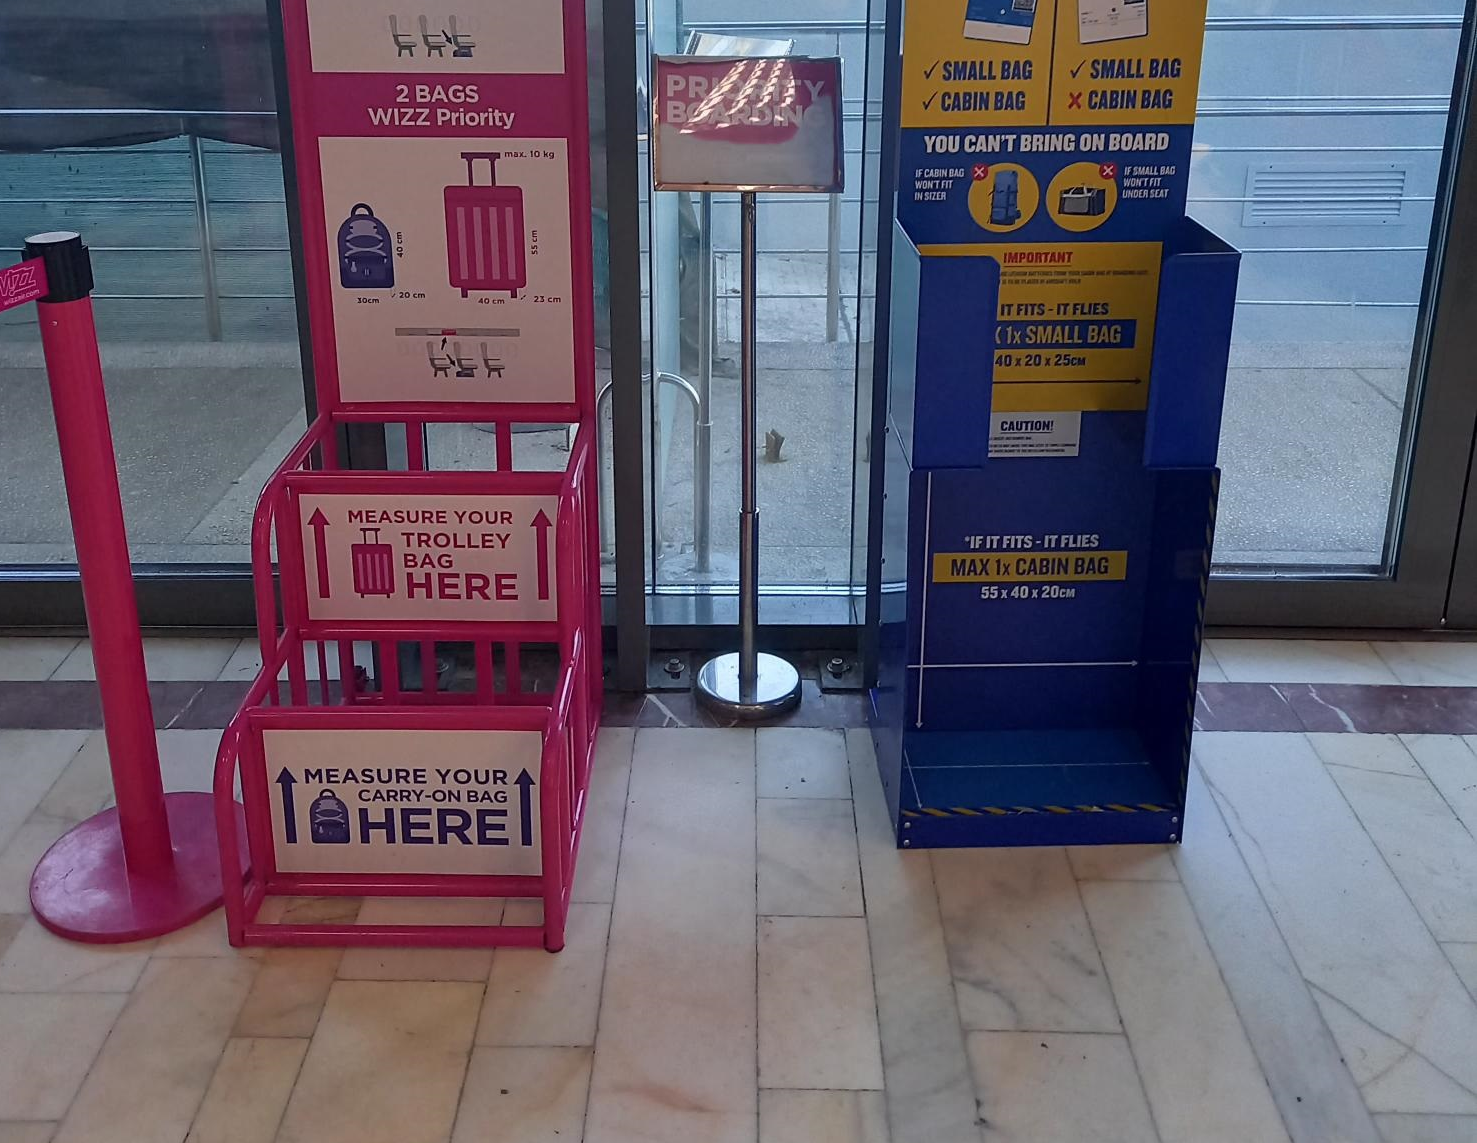
\includegraphics[width=0.42\textwidth]{luggage}%
	\hfill%
	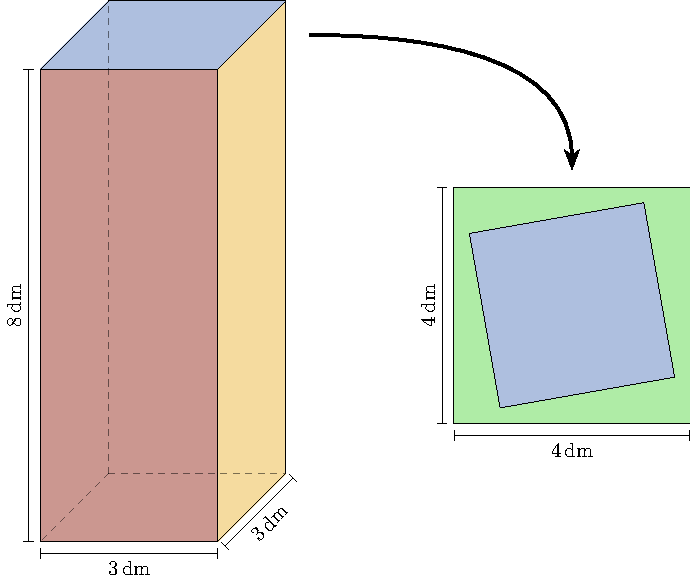
\includegraphics[width=0.42\textwidth]{sample2}%
\end{frame}

\begin{frame}[c]
	\frametitle{\problemtitle}
	\begin{block}{Solution}
		\begin{itemize}
			\item All sides of the largest box can always be covered with the same rectangle.
			\item For a given rectangle, the largest box has size $w\times h\times\min(w,h)$.
			\item Try all rectangles and take the maximum over all.
			\item[$\Rightarrow$] Runtime: $\mathcal{O}(n)$
		\end{itemize}
	\end{block}
	% \solvestats
\end{frame}